\section{理论框架：五维约束生命周期分类体系 (Schema v4)}
\label{sec:framework}

科学建模的首要前提在于：概念内涵的清晰界定先于实证评测的严谨性 \cite{lipton2019}。在当代风电预测文献中，将一个神经网络冠以“物理约束”之名，将数学形式截然不同、计算结构千差万别、工程依赖迥异的模型操作笼统混为一谈。为建立全流程实证审计的形式化理论基础，我们构建了\textbf{五维约束生命周期分类体系 (Schema v4)}。

\subsection{分析单元与生命周期表达}
在我们的分类体系中，实证审计的基本分析单元定义为预测模型流水线中所嵌入的\textbf{具体物理约束对象} $C$。当一篇发表文献同时集成多种截然不同的物理约束机制时（例如结合了气动功率经验曲线与空间尾流衰减模型），每个约束对象均被独立编码为一个生命周期实例。在形式上，我们将物理约束 $C$ 定义为一个跨越五个正交生命周期阶段的五元组：
\begin{equation}
C = \big\langle \mathcal{D}_1, \mathcal{D}_2, \mathcal{D}_3, \mathcal{D}_4, \mathcal{D}_5 \big\rangle,
\label{eq:constraint_tuple}
\end{equation}
其中 $\mathcal{D}_1$ 代表参数来源（Parameter Provenance），$\mathcal{D}_2$ 代表作用阶段（Application Stage），$\mathcal{D}_3$ 代表推理遥测依赖（Inference Telemetry Requirements），$\mathcal{D}_4$ 代表软件实现保真度（Implementation Software Fidelity），而 $\mathcal{D}_5$ 代表危害报告与消融有效性（Harm Reporting and Ablation Semantics）。从物理形式化规范到实际工业部署的生命周期全貌如图~\ref{fig:lifecycle}所示。

\begin{figure*}[!t]
\centering
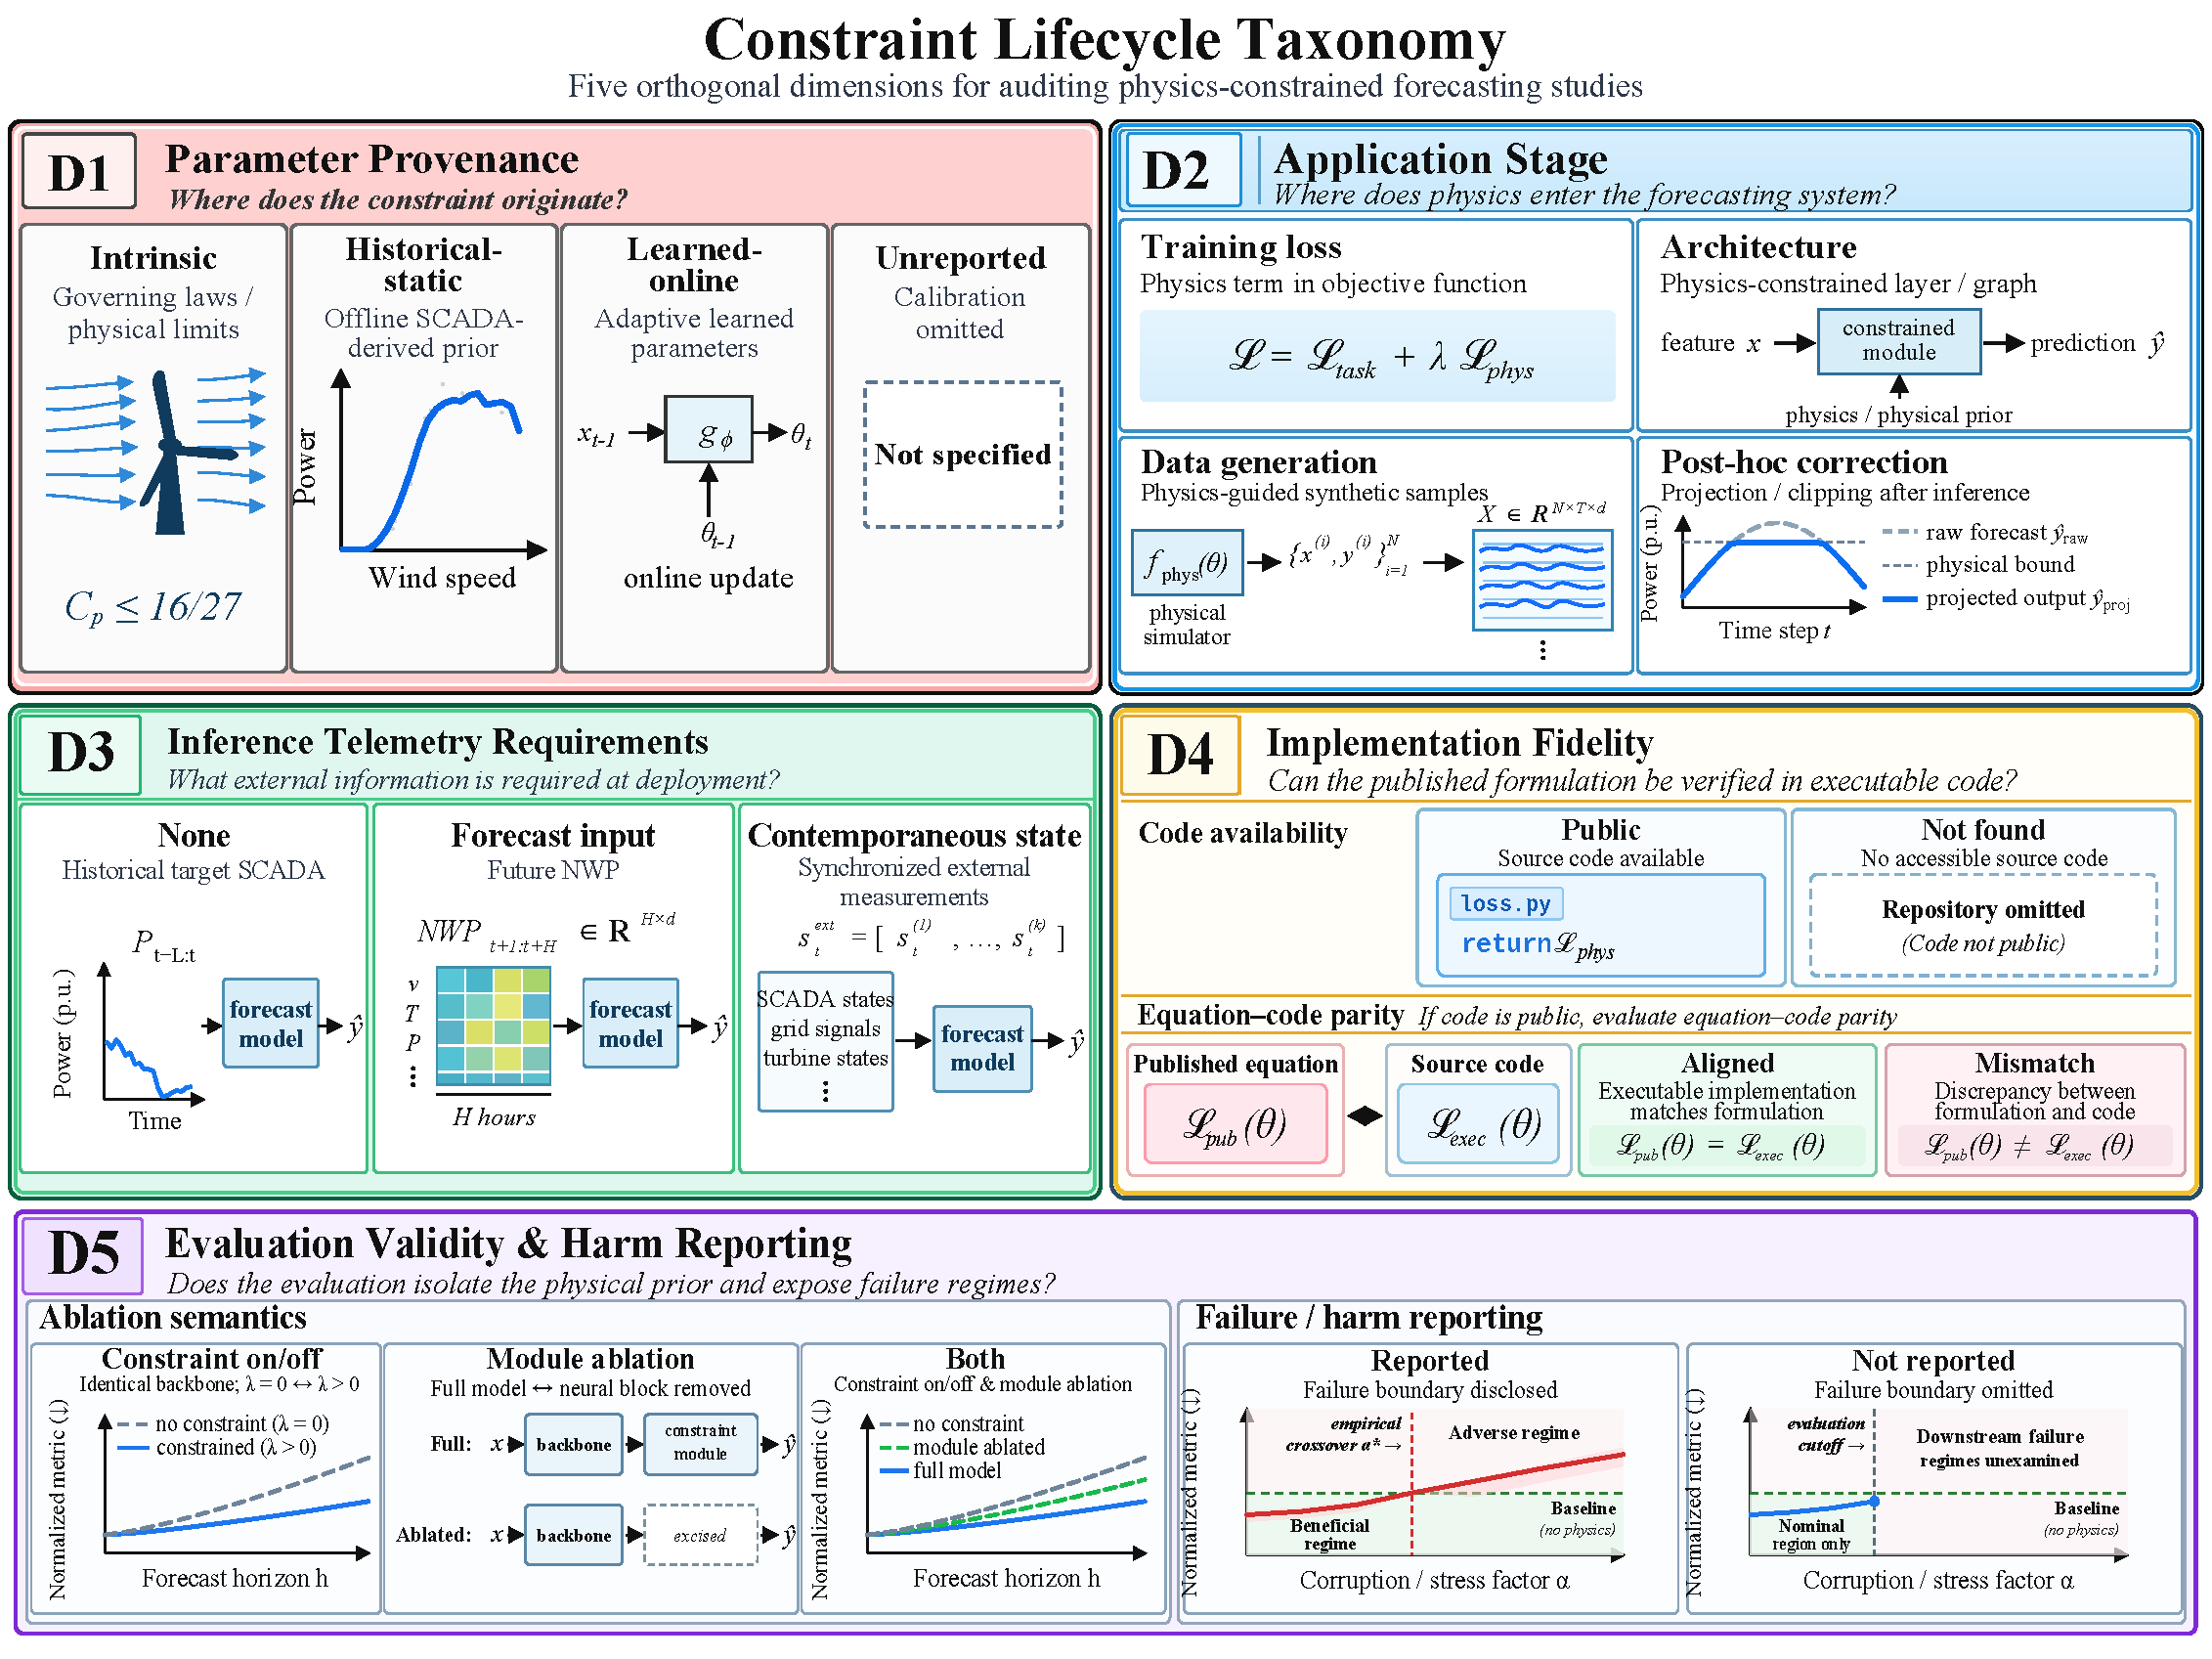
\includegraphics[width=\textwidth]{fig_constraint_lifecycle.pdf}
\caption{五维物理约束生命周期框架 (Schema v4)。系统追踪领域物理约束从数学机理来源 ($\mathcal{D}_1$)、计算图融入方式 ($\mathcal{D}_2$)、工业在线遥测依赖 ($\mathcal{D}_3$)、软件代码执行保真度 ($\mathcal{D}_4$) 到实证失效与消融有效性报告 ($\mathcal{D}_5$) 的全流程演进路径。}
\label{fig:lifecycle}
\end{figure*}

\subsection{五大生命周期维度的操作化定义}
Schema v4 通过五个正交维度对每个物理约束对象进行完备刻画：

\paragraph{维度 1：参数来源 ($\mathcal{D}_1$)}
该维度追踪约束数值参数的认识论起源与校准方式：
\begin{itemize}[leftmargin=1.5em,itemsep=1pt,topsep=2pt]
\item \textit{内生解析参数 (intrinsic)}：参数直接由第一性物理定律、出厂铭牌或经典方程推导，无需经验拟合（如 Betz 极限 $C_p \le 16/27$ 或经典运动学尾流方程）。
\item \textit{历史静态经验先验 (historical-static)}：参考曲线或分布由历史 SCADA 离线拟合并在推理中保持固定（如核密度估计经验流形）。
\item \textit{在线自适应学习参数 (learned-online)}：参数在推理期由辅助神经网络动态推断。
\end{itemize}
若文献未披露校准流程，归入\textit{未披露 (unreported)}。区分参数来源至关重要：静态经验先验隐式假定气动稳态，在机组老化或弃风限电时面临隐性失准风险。

\paragraph{维度 2：作用阶段 ($\mathcal{D}_2$)}
该维度界定物理知识介入深度学习流水线的具体计算环节：
(1)~\textit{训练损失正则化 (training-loss)}：物理先验作为可微惩罚项嵌入反向传播（$\mathcal{L} = \mathcal{L}_{\text{task}} + \lambda \mathcal{L}_{\text{phys}}$）；
(2)~\textit{推理架构约束 (inference-architecture)}：修改网络拓扑以严格限制前向输出可行域；
(3)~\textit{数据生成增强 (data-generation)}：在训练前用于合成或清洗数据；
(4)~\textit{事后投影滤波 (post-hoc-correction)}：推理完成后作为外置数学变换约束输出。

\paragraph{维度 3：推理遥测依赖 ($\mathcal{D}_3$)}
该维度识别在线部署时计算物理约束所需的外部实时数据流：
(1)~\textit{无外部依赖 (none)}：仅依赖目标机组历史功率自回归序列；
(2)~\textit{前瞻预测依赖 (forecast-input)}：必须输入未来气象预报（如数值天气预报风向风速）；
(3)~\textit{同期状态依赖 (contemporaneous-state)}：前向推理需要来自临近机组或测风塔的无延迟同步物理测量。
关键的逻辑区分在于：$\mathcal{D}_3 = \texttt{none}$ 仅界定基准预测模型本身不需要外部实时数据流（如测风塔实时遥测或前瞻数值天气预报）。然而，若某一物理约束机制在测试推理期依赖外部气象物理代理（例如利用风速输入检索经验静态功率曲线先验），而实际现场又缺乏前瞻数值天气预报或零延迟传感器时，工程部署将被迫在测试推理期剔除约束或以存在滞后的历史观测代偿。因此，观测陈旧度（observation staleness）是依赖物理代理的约束架构在现实遥测延迟下的实证运行隐患，而非 $\mathcal{D}_3 = \texttt{none}$ 分类所内生的必然推论。

\paragraph{维度 4：实现保真度 ($\mathcal{D}_4$)}
该维度评估公开软件是否忠实执行已发表论文的数学规范：
(1)~\textit{验证对齐 (verified-aligned)}：公开代码经审查证实与论文公式完全相符；
(2)~\textit{代码失配 (code-mismatch)}：公开代码在代数形式或参数方向上偏离论文公式；
(3)~\textit{未找到代码 (not-found)}：未提供公开仓库或执行脚本。
数学排版常掩盖数值执行差异，使得静态代码审计成为不可或缺的复核手段。

\paragraph{维度 5：危害报告与消融语义 ($\mathcal{D}_5$)}
该维度审查实证评估是否因果隔离了物理约束本身：
(1)~\textit{严格隔离消融 (strict-isolation)}：基准与实验组参数容量完全对齐，仅改变物理先验权重（$\lambda=0$ vs.\ $\lambda>0$）；
(2)~\textit{粗粒度模块消融 (module-ablation)}：直接切除多层神经网络子模块，混淆参数容量与领域先验；
(3)~\textit{兼具两者 (both)}：同时报告参数隔离与模块切除；
(4)~\textit{危害报告 (harm-reported)}：显式量化约束导致性能劣化的运行边界。

\subsection{消歧准则与体系形式化一致性}
为确保多位独立评分员在分类编码中达成高复现性，Schema v4 确立了三项基础消歧准则。参数来源（$\mathcal{D}_1$）严格独立于测试期遥测（$\mathcal{D}_3$）：离线标定参数所用的历史数据，与在线推理所需的实时数据流在工程上相互独立。作用阶段（$\mathcal{D}_2$）依据梯度反向传播路径进行严格判定：仅在反向传播中施加损失惩罚的归入训练期损失正则化，在网络随机初始化下仍能限制前向计算域的归入推理期架构约束。因果消融（$\mathcal{D}_5$）必须采用严格参数匹配的对照基准：直接移除多层神经网络子模块反映的是网络整体表征容量的变动，无法作为物理先验的独立因果依据。
